\chapter{Experimental Validation}
\label{sec:ExperimentalValidation}


\begin{figure}[htp]
	\centering
		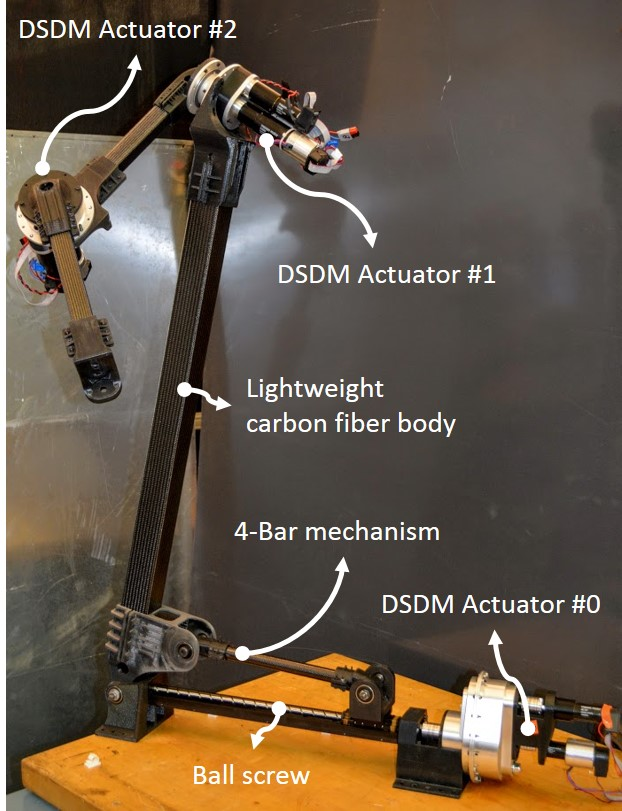
\includegraphics[width=0.60\textwidth]{arm_proto_3.jpg}
	\caption{3-DoF custom arm using 3 DSDM actuators}
	\label{fig:dsdm_arm}
\end{figure}


\section{DSDM-arm}
\label{sec:DSDMArm}

\subsection{Actuator design}
\label{sec:ActuatorDesign}

\begin{figure}[htp]
	\centering
		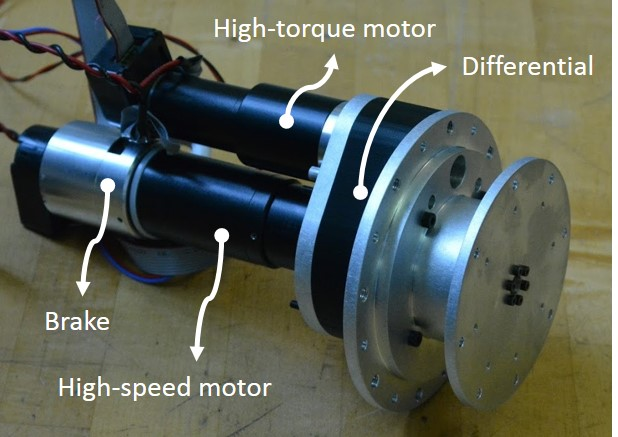
\includegraphics[width=0.75\textwidth]{dsdm_proto_2.jpg}
	\caption{Revolute joint DSDM actuator prototype } %Max continuous torque of 40 Nm and maximum velocity of 100 RPM
	\label{fig:dsdm_act}
\end{figure}



\subsection{Arm design}
\label{sec:ArmDesign}


Shown in Fig. \ref{fig:arm_proto}, a 3-DoF robotic arm using variable gear-ratio actuators has been designed and custom built. The variable gear-ratio actuators consist of dual-speed dual-motor (DSDM) actuators, as shown in Fig. \ref{fig:dsdm_cad}. Those actuators have two discrete operating modes, one for high-speed operation, and the other for low-speed, high-load operation, where the net gear-ratios are more than 20-times different. DSDM actuators are lighter than would be single motors sized to reach the same maximum speed and maximum torque \cite{girard_two-speed_2015}. Also, the dual-motor architecture has the advantages of allowing fast and seamless gear-shifts, by doing the synchronization in the nullspace, which support the modeling assumption discussed at sec. \ref{sec:mod}. 


%For instance, the actuation and joint unit shown at Fig. \ref{fig:dsdm_cad} weights 1.5 Kg (un-optimized first prototype), can reach a 100 RPM velocity and a maximum continuous torque of 40 Nm (based on the very conservative torque rating of Maxon motor [ref] )

%\begin{figure}[htp]
	%\centering
		%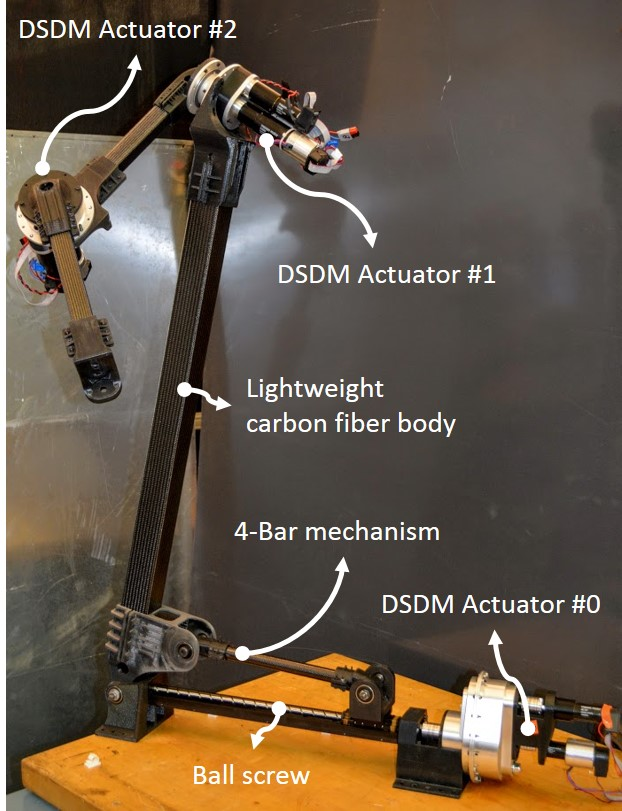
\includegraphics[width=0.45\textwidth]{arm_proto_3.jpg}
	%\caption{Prototype 3-DOF arm with variable gear-ratio actuators}
	%\label{fig:arm_proto}
%\end{figure}



\subsection{Control software architecture}
\label{sec:ControlSoftwareArchitecture}

The control algorithms are implemented on a computer using ROS \cite{quigley_ros:_2009}, the trajectory generation algorithm and the R* Computed Torque controller are written in \textit{Python}. The computer is communicating over USB with open-source \textit{Flexsea} motor-drivers \cite{duval_flexsea-execute:_2016} that handle the low-level current loops. The trajectory is generated offline in advance and loaded in memory upon initialization. The main R* control loop is running at a 500 Hz sampling rate. The low-level actuator controllers, receiving the torque and gear-ratio set-points, communicating with both motor drivers and handling the gear-shifting process (see Fig. \ref{fig:control_achitecture}), are also implemented in \textit{Python} and use the algorithm described in \cite{girard_two-speed_2015}. Transition from one gear-ratio to another are found to be consistently under 50 ms.


\section{Experimental results}
\label{sec:ExperimentalResults}




\subsection{Seamless gearshifts}
\label{sec:SeamlessGearshifts}

\subsection{Dynamic motions}
\label{sec:DynamicMotions}


Here a trajectory following experiments using the last DoF of the robot only is presented. A 1.5 Kg load is mounted on the end-effector, and the task is to bring it from the bottom position ($q=-\pi$) to the up-right position ($q=0$) using as little torques as possible. An RRT trajectory planning algorithm is used to search for a low torque trajectory reaching the goal, see Fig. \ref{fig:exp_rrt}. Then the R* Computed Torque Controller is used to track the reference trajectory. The experimental results are shown in Fig. \ref{fig:exp_traj} and a video of this experiment is also available in the multimedia attachment. 
%
\begin{figure}[htp]
	\centering
		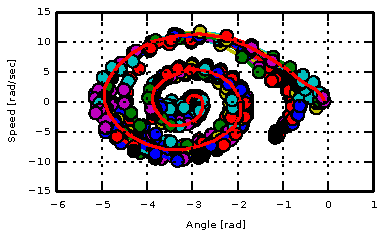
\includegraphics[width=0.43\textwidth]{rrt_fig.pdf}
	\caption{Trajectory generation algorithm searching for a low torque solution}
	\label{fig:exp_rrt}
\end{figure}
%
\begin{figure}[htp]
	\centering
		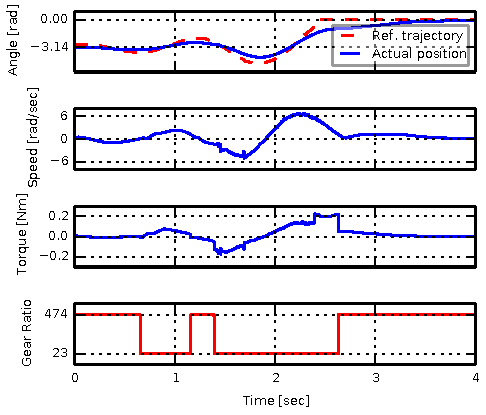
\includegraphics[width=0.45\textwidth]{exp_fig3.pdf}
	\caption{Experimental results}
	\label{fig:exp_traj}
	\vspace{-10pt}
\end{figure}
%
Results show that the robot is using its 1:23 gear-ratio to accumulate kinetic energy by swinging the arm link back and forth. Also the R* controller selects the 1:474 gear-ratio automatically to attenuate the load dynamics, when the actuator has to force the robot to stay with the trajectory.  Interestingly, the reference trajectory was planned so the robot would accumulate enough kinetic energy to swing straight up with the last swing. However, in the experiment, the dissipative forces are greater than anticipated by the planner, and the last swing is too small (the robot almost stop at $q=-0.9$ at $t=2.6$ in Fig. \ref{fig:exp_traj}). Then, the R* controller automatically engage the large 1:474 gear-ratio, to continue converging on the desired trajectory with much smaller torques than those required if keeping using the 1:23 gear-ratio in this situation (no momentum and a large gravitational force to overpower). This illustrates that including the gear-ratio selection in the feedback loop also increase the robustness of the system. Without the 1:474 gear-ratio option, tracking would have failed as the computed torque with 1:23 in this situation was greater than the maximum allowable motor torque.


